\documentclass[10pt,UTF8]{ctexart}


\usepackage[margin=2cm,a4paper]{geometry}
%\usepackage[left=0.75in,top=0.6in,right=0.75in,bottom=1.0in,a4paper]{geometry}

\setmainfont{Caladea}
%% 也可以選用其它字庫:
% \setCJKmainfont[%
%   ItalicFont=AR PL KaitiM GB,
%   BoldFont=Noto Sans CJK SC,
% ]{Noto Serif CJK SC}
% \setCJKsansfont{Noto Sans CJK SC}
% \renewcommand{\kaishu}{\CJKfontspec{AR PL KaitiM GB}}

% 繁體中文
\setCJKmainfont[Path=fonts/ ]{NotoSansTC-Medium.otf}

\usepackage{minted}
\usepackage[breaklinks]{hyperref}

% Picture
% 導言區的此三行無變化
\usepackage{graphicx}
\usepackage{float} 
\usepackage{subfigure}
% 以下是新增的自定義格式更改
\usepackage[]{caption2} %新增調用的宏包
\renewcommand{\figurename}{Fig.} %重定義編號前綴詞
\renewcommand{\captionlabeldelim}{.~} %重定義分隔符
 %\roman 是羅馬數字編號,\alph是默認的字母編號,\arabic是阿拉伯數字編號,可按需替換下一行的相應位置
\renewcommand{\thesubfigure}{(\roman{subfigure})}%此外,還可設置圖編號顯示格式,加括號或者不加括號
\makeatletter \renewcommand{\@thesubfigure}{\thesubfigure \space}%子圖編號與名稱的間隔設置
\renewcommand{\p@subfigure}{} \makeatother

% Math
\usepackage {mathtools}
\usepackage{amssymb}

% Code
\usepackage{listings}
\usepackage{xcolor}
\lstset{
    % backgroundcolor=\color{red!50!green!50!blue!50},
    % 程式碼塊背景色為淺灰色
    rulesepcolor= \color{gray}, % 程式碼塊邊框顏色
    breaklines=true,  % 程式碼過長則換行
    numbers=left, % 行號在左側顯示
    numberstyle= \small,% 行號字型
    % eywordstyle= \color{red,% 關鍵字顏色
    commentstyle=\color{gray}, % 註釋顏色
    frame=shadowbox % 用方框框住程式碼塊
    }

\usepackage{hyperref}

\title{數字媒體軟件與系統開發}
\author{干皓丞,2101212850, 信息工程學院}

\begin{document}
\maketitle


\section{作業目標與章節摘要}

下載 GPAC,理解並描述 random access 過程。

\begin{figure}[H]
\centering 
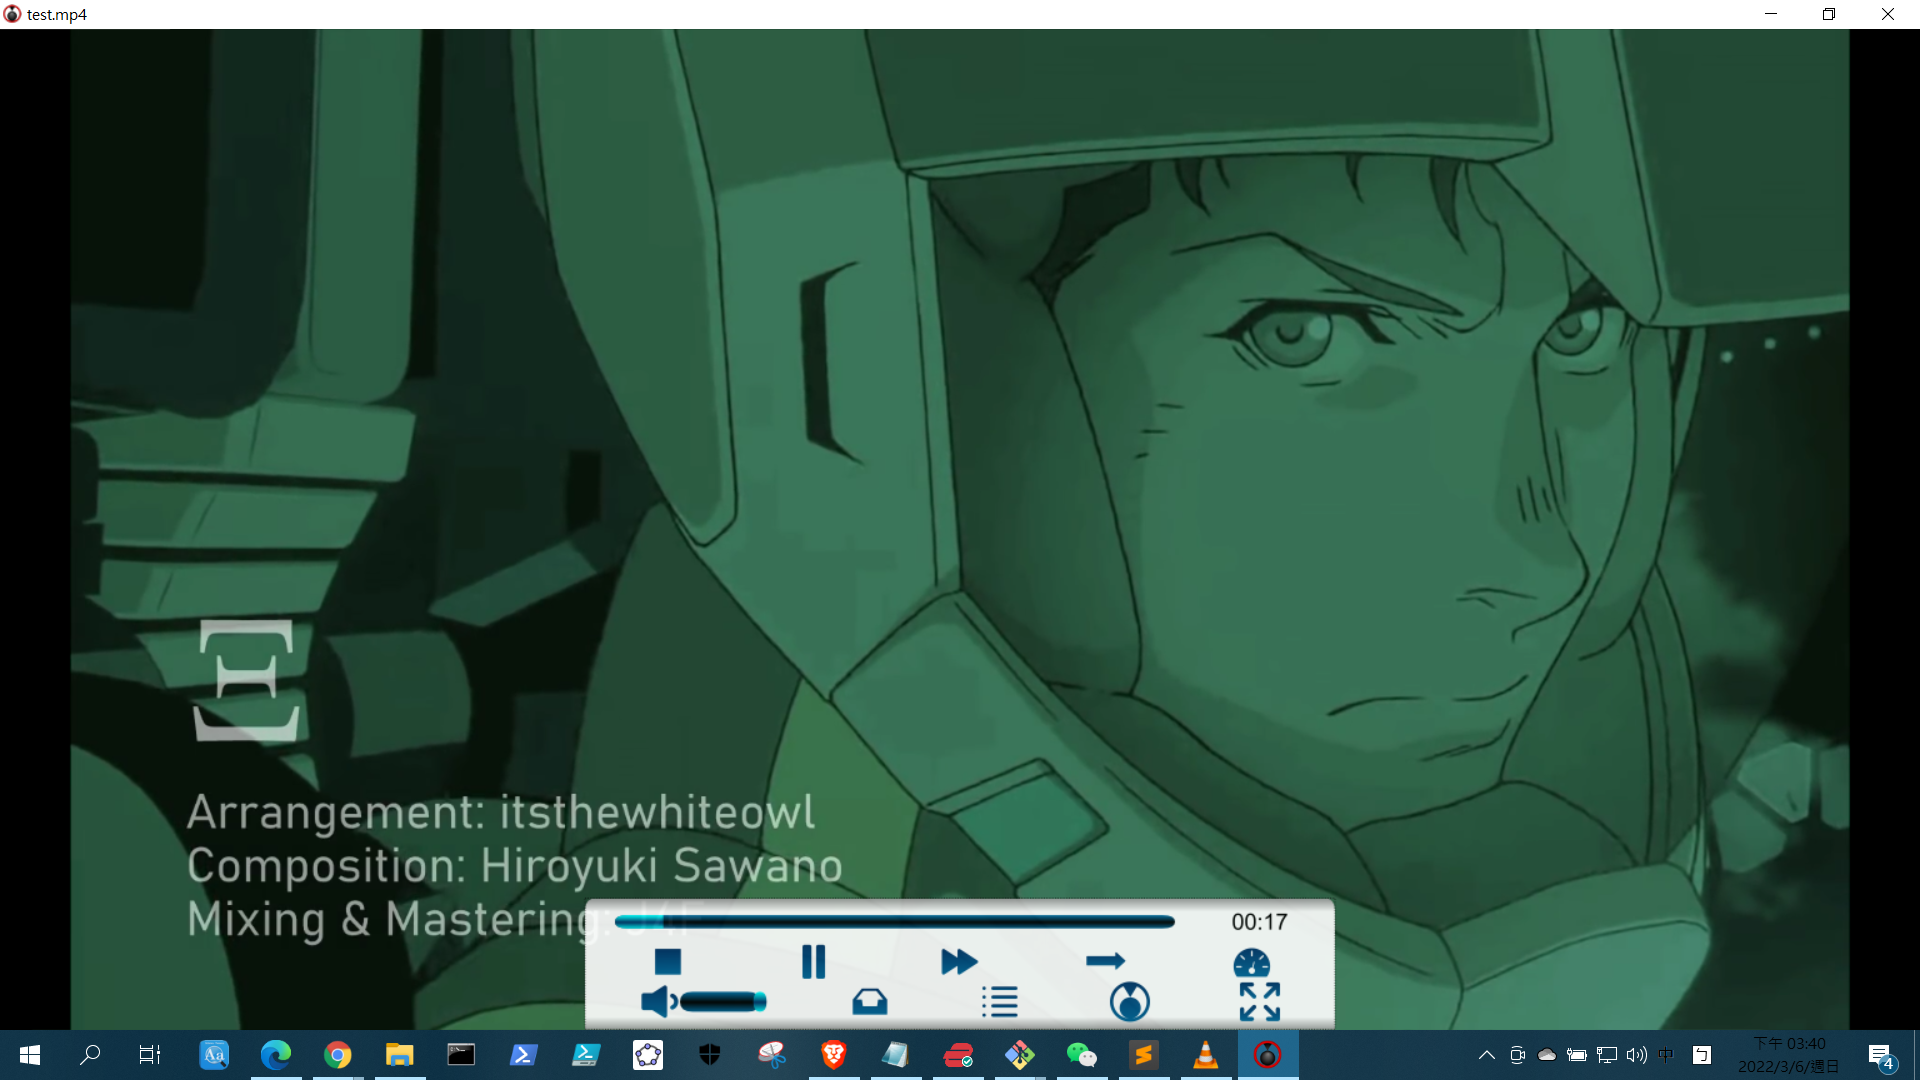
\includegraphics[width=0.80\textwidth]{g2.png} 
\caption{使用安裝好的 GPAC 的 Osmo4 播放}
\label{Test}
\end{figure}


\section{文章與作業狀況}

作業可以從 GitHub 下的 kancheng/kan-cs-report-in-2022 專案找到,作業程式碼與文件目錄為 kan-cs-report-in-2022/DMSASD/gpac-random-access。實際執行的環境與實驗設備為 Google 的 Colab 、MacBook Pro (Retina, 15-inch, Mid 2014) 、 Acer Aspire R7 與 HP Victus (Nvidia GeForce RTX 3060)。


\section{作業內容概述}

此作業分二大部分,第一部分說明 GPAC 使用與理解,第二部分則描述描述 Random Access 過程。

1. GPAC 使用與理解

2. 描述 Random Access 過程

\section{GPAC 使用與理解}

GPAC 是一個 LGPL v2.1 且在大多數情況下也可以在商業許可下使用的開源多媒體框架,其專案提供了使用者在處理、檢查、打包、流式傳輸、播放和與媒體內容交互的工具。此類內容可以為音頻、影像、字幕、元數據、可縮放圖形、加密媒體、2D/3D 圖形和 ECMAScript 等任意組合。GPAC 以其廣泛的 MP4/ISOBMFF 功能而聞名,深受影像愛好者、學術研究人員、標準化機構和專業廣播公司的歡迎。

前往 GPAC (https://gpac.wp.imt.fr/) 下載,安裝後即可以使用。開啟終端機查看版本。

1. GPAC 的官方開發文件: https://doxygen.gpac.io/

2. GPAC 的 Wiki: https://github.com/gpac/gpac/wiki/Howtos

\begin{figure}[H]
\centering 
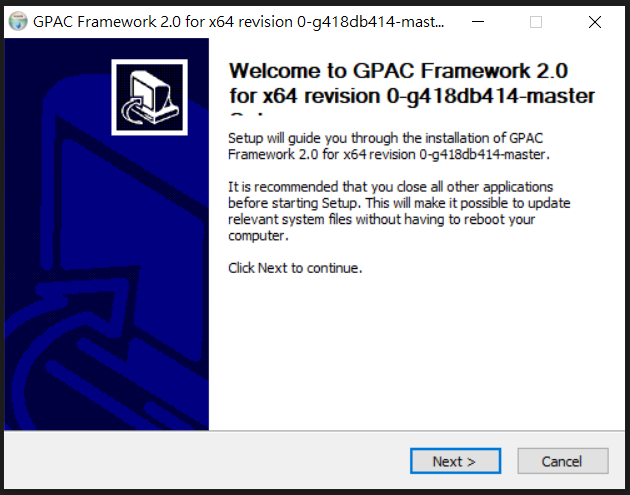
\includegraphics[width=0.80\textwidth]{g1.png} 
\caption{在此使用 GPAC 的 Windows 版本安裝}
\label{Test}
\end{figure}

\begin{figure}[H]
\centering 
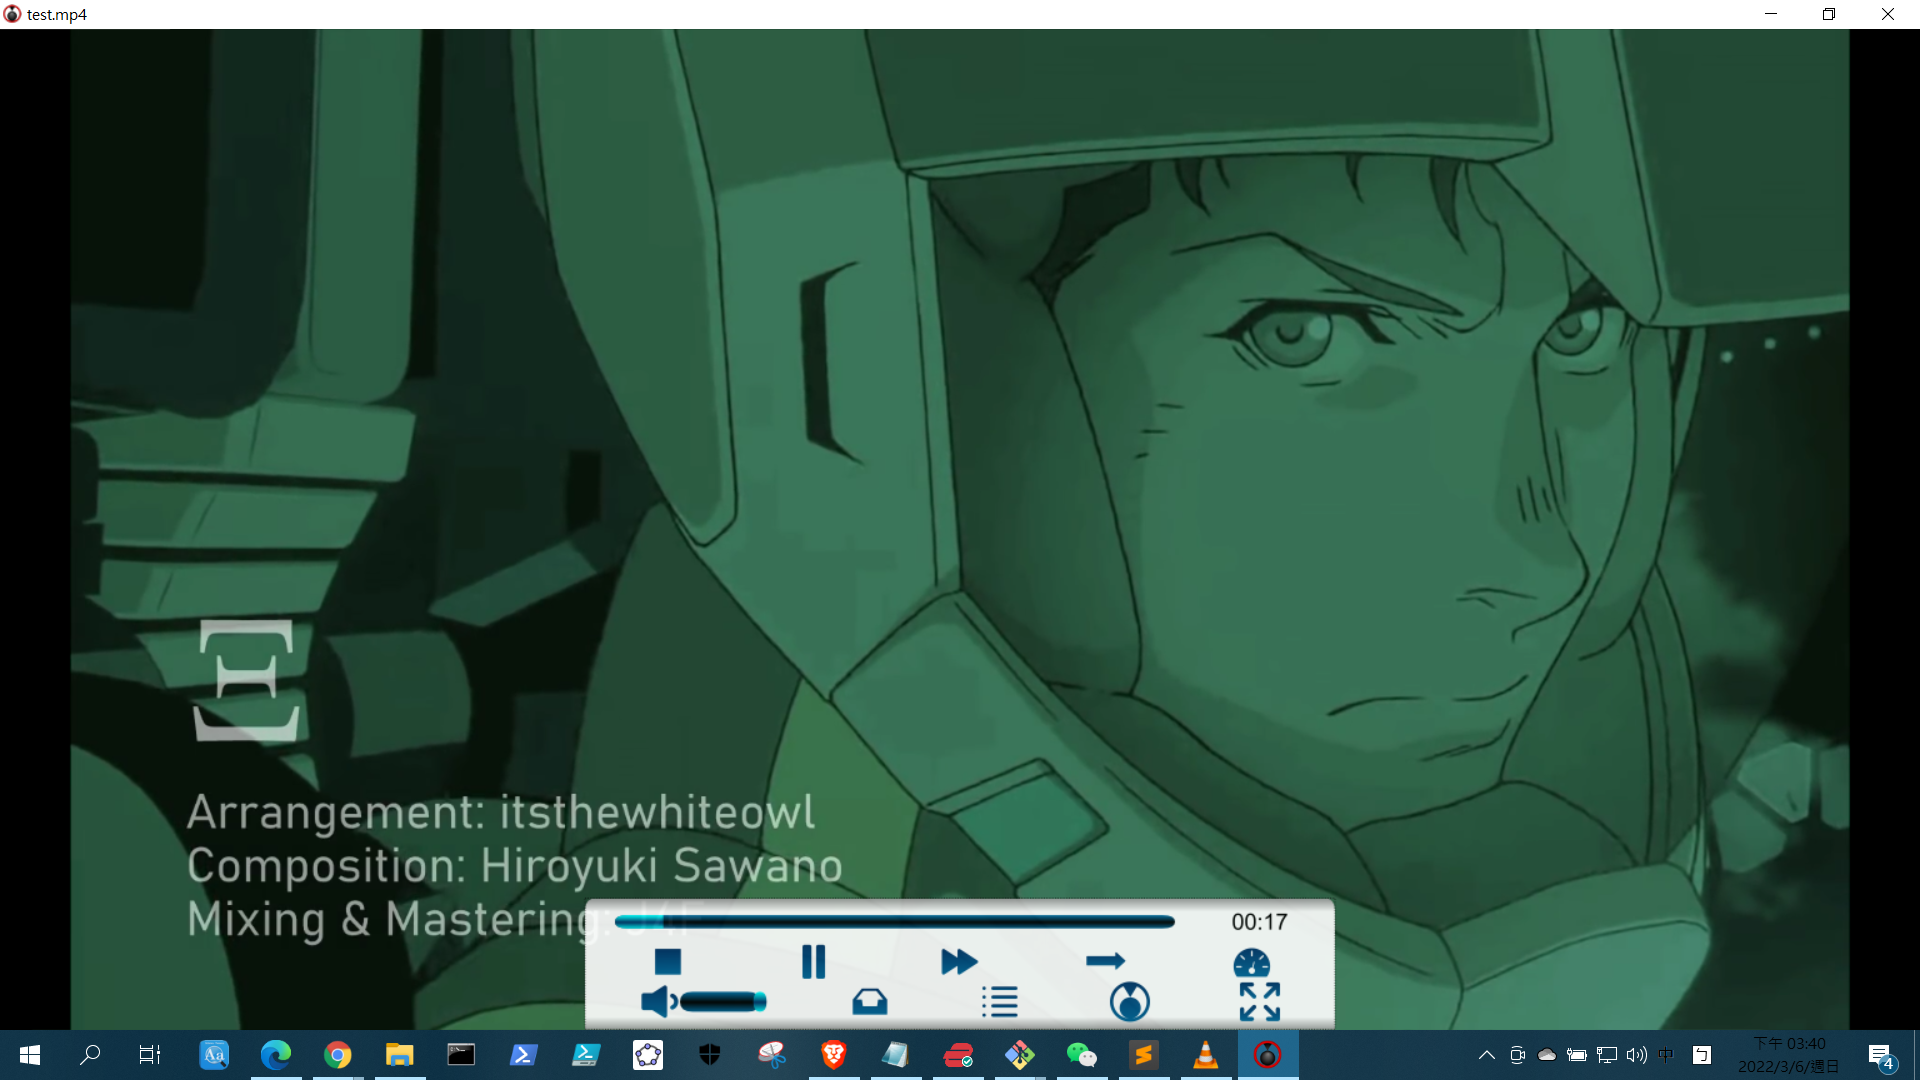
\includegraphics[width=0.80\textwidth]{g2.png} 
\caption{完成}
\label{Test}
\end{figure}

1. 查看 mp4box 版本

\begin{lstlisting}[language={python}]
mp4box -version
\end{lstlisting}

\begin{figure}[H]
\centering 
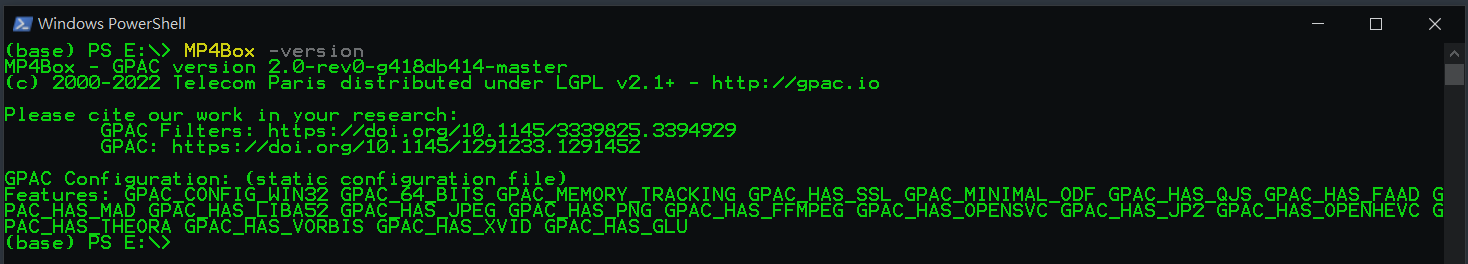
\includegraphics[width=0.80\textwidth]{g3.png} 
\caption{查看 GPAC 的  mp4box 版本}
\label{Test}
\end{figure}

2. 查看 mp4box 操作指令

\begin{lstlisting}[language={python}]
# 1
mp4box -h
# 查看 mp4box 中的所有幫助信息

# 2
mp4box -h general
# 查看 mp4box 中的通用幫助信息

# 3
mp4box -info test.mp4 
# 查看 test.mp4 文件是否有問題

# 4
mp4box -add test.mp4 test-new.mp4
# 修復 test.mp4 文件格式不標準的問題,並把新文件保存在 test-new.mp4 中

# 5
mp4box  -inter  10000 test-new.mp4 
# 解決開始播放 test-new.mp4 卡一下的問題,為 HTTP 下載快速播放有效,10000ms

# 6
mp4box -add file.avi new_file.mp4
# 把 avi 文件轉換為 mp4 文件

# 7
mp4box -hint file.mp4 
# 為 RTP 準備,此指令將為文件創建RTP提示跟踪信息。
# 這使得經典的流媒體服務器像 darwinstreamingserver 或 QuickTime 的流媒體服務器通過 RTSP/RTP 傳輸文件

# 8
mp4box -cat test1.mp4 -cat test2.mp4 -new test.mp4 
# 把 test1.mp4 和 test2.mp4 合併到一個新的文件 test.mp4 中,要求編碼參數一致

# 9
mp4box -force-cat test1.mp4 -force-cat test2.mp4 -new test.mp4 
# 把 test1.mp4 和 test2.mp4 強制合併到一個新的文件 test.mp4 中,有可能不能播放

# 10
mp4box -add video1.264 -cat video2.264 -cat video3.264 -add audio1.aac -cat audio2.aac -cat audio3.aac -new muxed.mp4 -fps 24 
# 合併多段音視頻並保持同步 

# 11
mp4box -split *time_sec* test.mp4
# 切取 test.mp4 中的前面 time_sec 秒的視頻文件

# 12
mp4box -split-size *size *test.mp4 
# 切取前面大小為 size KB的視頻文件

# 13
mp4box -split-chunk *S:E* test.mp4 
# 切取起始為 S 少,結束為 E 秒的視頻文件

# 14
mp4box -add 1.mp4#video -add 2.mp4#audio -new test.mp4
# test.mp4 由 1.mp4 中的視頻與 2.mp4 中的音頻合併生成
\end{lstlisting}

\section{描述 Random Access 過程}


\begin{figure}[H]
\centering 
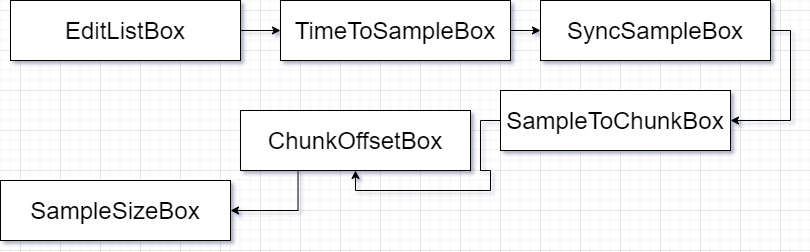
\includegraphics[width=0.80\textwidth]{g8.png} 
\caption{描述 Random Access 過程圖}
\label{Test}
\end{figure}

If you want to seek a given track to a time T,

假如想要最一個文件進行隨機訪問,而該訪問進行為 T 時刻 EX : 第三分五十秒。

1. If the track contains an edit list, determine which edit contains the time T by iterating over the edits. T\_movie = T\_start + T’

如果軌道包含編輯列表,則通過迭代編輯確定哪個編輯包含時間 T。 T\_movie = T\_start + T'

先找當中有沒有 edit list,當中 edit list 實際上存著一段段的樣本信息,這裡面會有一個關鍵字段的有開始時刻(T\_start)的連續樣本。這個過程就是將 T 換算成 T\_start + T',而這個 T' 就是換算出來的新的時間。

2. Convert to media time scale T\_media = T\_start’ + T’’

然後再將原先的過程轉換為媒體時間尺度 T\_media = T\_start' + T''


3. Use time-to-sample box to find the first sample prior to the given time

使用 time-to-sample box 找到給定時間之前的第一個樣本,也就是對應的樣本編號。

4. Consult the sync sample table to seek to which sample is closest to, but prior to, the sample found above

因為找到的樣本不一定是可以解的,為了保險會先查閱同步樣本表以尋找最接近但先於上面所找到的樣本的樣本編號。

5. Use the sample-to-chunk table to determine in which chunk this sample is located.

使用 sample-to-chunk 來確定該樣本位於哪個 chunk 中。

6. use the chunk offset box to figure out where that chunk begins

找到後根據使用 the chunk offset box 來確定該 chunk 開始的物理存儲位置。

7. Starting from this offset, you can use the information contained in the sample-to-chunk box and the sample size box to figure out where within this chunk the sample in question is located.

從這個偏移量開始,您可以使用包含在 sample-to-chunk box 和 the sample size box 中的信息來確定有問題的樣本在這個 chunk 中的位置。

尋找專案中有關 Random Access 的部分,利用 find 和 grep 指令,尋找 GPAC 與 Random Access 過程有關的檔案。


\begin{lstlisting}[language={python}]
find . -name "*.*" |xargs grep "random access" *.*
\end{lstlisting}

\begin{figure}[H]
\centering 
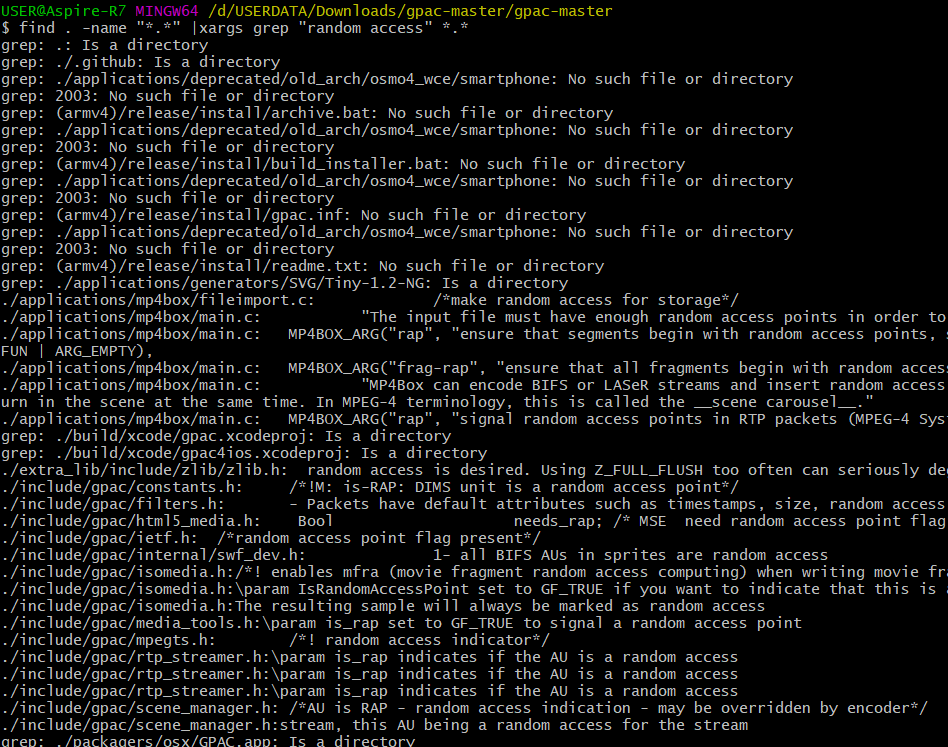
\includegraphics[width=0.80\textwidth]{g6.png} 
\caption{尋找 GPAC 與 Random Access 過程有關的檔案}
\label{Test}
\end{figure}

\begin{lstlisting}[language={python}]
./applications/mp4box/fileimport.c
./applications/mp4box/main.c
./extra_lib/include/zlib/zlib.h
./include/gpac/constants.h
./include/gpac/filters.h:
./include/gpac/html5_media.h:
./include/gpac/ietf.h:
./include/gpac/internal/swf_dev.h:
./include/gpac/isomedia.h:
./include/gpac/isomedia.h:
./include/gpac/media_tools.h:
./include/gpac/mpegts.h:
./include/gpac/rtp_streamer.h:
./include/gpac/scene_manager.h: 
./share/doc/man/gpac-filters.1:mfra (bool, default: false):
./share/doc/man/mp4box.1:
./src/filters/mux_isom.c:
./src/media_tools/html5_mse.c: 
./src/media_tools/m2ts_mux.c:
./src/scene_manager/text_to_bifs.c:
\end{lstlisting}

同時可以從 GPAC 的官方文件看到 Random Access 的部分。

\begin{figure}[H]
\centering 
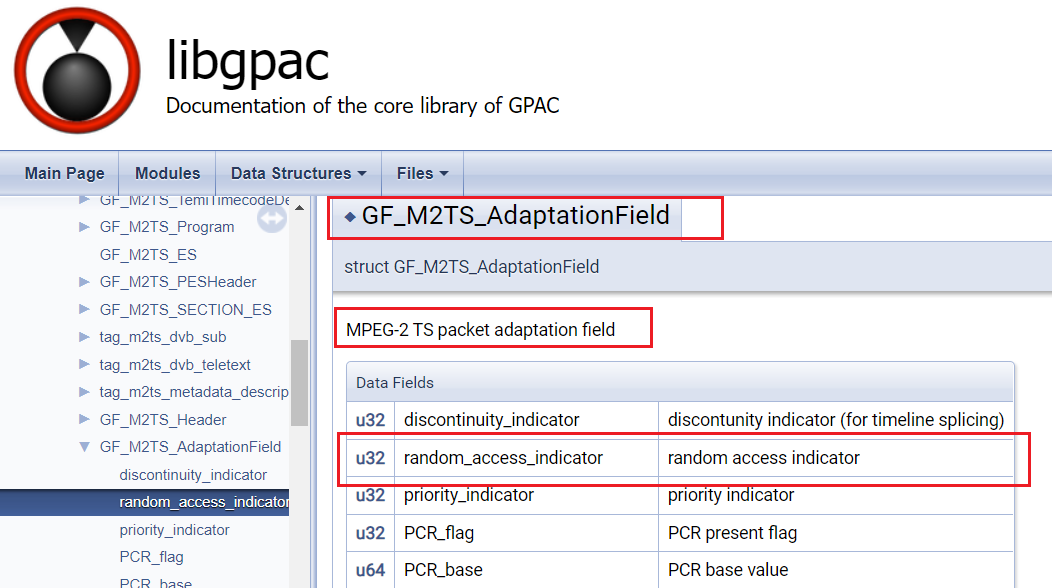
\includegraphics[width=0.80\textwidth]{g7.png} 
\caption{文件 GPAC 與 Random Access }
\label{Test}
\end{figure}

%\section{附錄}

% 數學意義說明

% $$\min \limits_{G}\max \limits_{D}{V_I(D,\ G)=V(D,G)-\lambda L_I(G,Q)}$$

%	\begin{lstlisting}[language={python}]

%	\end{lstlisting}

%\begin{enumerate}
%\item Y
%\item A
%\end{enumerate}

% \newpage

\clearpage

\end{document}